%%%%%%%%%%%%%%%%%%%%%%%%%%%%%%%%%%%%%%%%%
% fphw Assignment
% LaTeX Template
% Version 1.0 (27/04/2019)
%
% This template originates from:
% https://www.LaTeXTemplates.com
%
% Authors:
% Class by Felipe Portales-Oliva (f.portales.oliva@gmail.com) with template 
% content and modifications by Vel (vel@LaTeXTemplates.com)
%
% Template (this file) License:
% CC BY-NC-SA 3.0 (http://creativecommons.org/licenses/by-nc-sa/3.0/)
%
%%%%%%%%%%%%%%%%%%%%%%%%%%%%%%%%%%%%%%%%%

%----------------------------------------------------------------------------------------
%	PACKAGES AND OTHER DOCUMENT CONFIGURATIONS
%----------------------------------------------------------------------------------------

\documentclass[
	12pt, % Default font size, values between 10pt-12pt are allowed
	%letterpaper, % Uncomment for US letter paper size
	%spanish, % Uncomment for Spanish
]{fphw}

% Template-specific packages
\usepackage[utf8]{inputenc} % Required for inputting international characters
\usepackage[T1]{fontenc} % Output font encoding for international characters
\usepackage{mathpazo} % Use the Palatino font

\usepackage{graphicx} % Required for including images

\usepackage{booktabs} % Required for better horizontal rules in tables

\usepackage{listings} % Required for insertion of code

\usepackage{enumerate} % To modify the enumerate environment

\usepackage{caption}

\usepackage{listings}

\usepackage{float}

\usepackage{relsize}
\usepackage{xcolor}

\definecolor{mygreen}{rgb}{0,0.6,0}
\definecolor{mygray}{rgb}{0.5,0.5,0.5}

\lstset{language=Python,%
	%basicstyle=\color{red},
	breaklines=true,%
	keywordstyle=\color{blue},
	morekeywords=[2]{1}, keywordstyle=[2]{\color{black}},
	identifierstyle=\color{black},
	stringstyle=\color{gray},
	commentstyle=\color{mygreen},
	numberstyle=\tiny\color{mygray}, % the style that is used for the line-numbers
           rulecolor=\color{black},
	showstringspaces=false,
	emph=[1]{for,end,break},emphstyle=[1]\color{green},
	}

%----------------------------------------------------------------------------------------
%	ASSIGNMENT INFORMATION
%----------------------------------------------------------------------------------------

\title{Deep Learning on Kubeflow} % Assignment title

\author{ Iurii Mozzhurin \& Rebekka Pech} % Student name

\date{July 28th, 2019} % Due date

\institute{Goethe University Frankfurt am Main}% \\ Big Data Lab} % Institute or school name

\class{Hands-on Lab - Big Data Technologies SS 2019} % Course or class name

%----------------------------------------------------------------------------------------

\begin{document}

\maketitle % Output the assignment title, created automatically using the information in the custom commands above

%----------------------------------------------------------------------------------------
%	ASSIGNMENT CONTENT
%----------------------------------------------------------------------------------------

\vspace{50pt}

\section{Introduction to Kubeflow}

\noindent Kubeflow is an open source platform which is based on Kubernetes and was developed by Google. It's dedicated for making deployments of Machine Learning workflows on Kubernetes simple, portable (it works on any Kubernetes cluster) and scalable (upon need). Kubeflow makes it possible to bring ML in any existing cluster. \\

\noindent When talking about Kubeflow you also have to talk about Kubernetes. Kubernetes is an open-source container-orchestration system. With Kubernetes you only need to define what resources the app needs, how many instances should be made, and Kubernetes takes care of deploying, managing and balancing containers on the hardware (nodes).\\  

\noindent The main idea of Kubeflow is that it's a ready-to-use set of Machine Learning tools. It's not necessary to install and connect the tools separately, but it can be done automatically. It also provides GUI, which makes the work with them easy for non-programmers.\\
Kubeflow includes components for model developing, training and serving and also for hyperparameter tuning and pipelines.\\
Kubeflow should be used for distributed ML workflow, for ML in production or for ML in cloud.
\ \\
%%%%%%%%%%%%%%%%%%%%%%%%%%%%%%%%%%%%%%%%%%%%%%%%%%
%\newpage
\section{Use Case Setup}

\noindent The intention of our use case was to train a CNN model to distinguish between works of ten
painters. In the end we wanted to have a (good) prediction when we give an image into our model whose painting it is.\\

\noindent For this model we used the Dataset ``Painter by Numbers'' from kaggle.com which has an original size of 83GB  but that includes a lot of images from much more than 10 artists. Most of the images were from WikiArt.org.\\
 In the original dataset we had Image dimensions from 477 to 7444 Pixels.\\

\begin{figure}[H]
	\center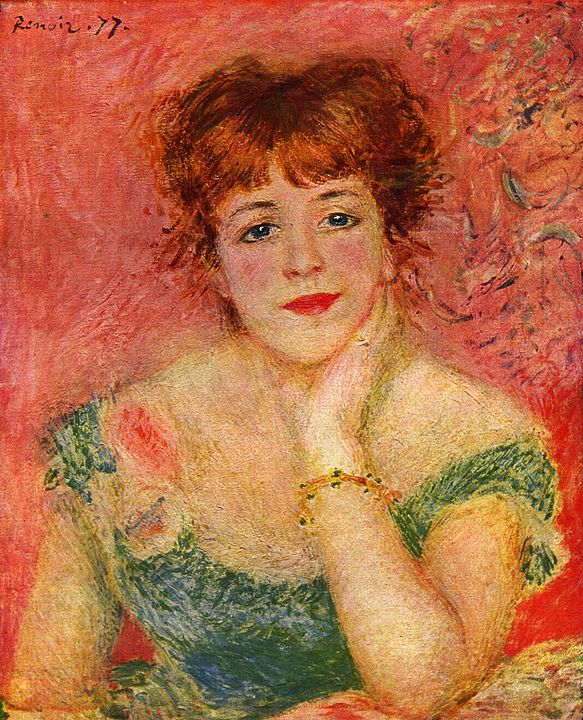
\includegraphics[width=0.2 \textwidth]{Renoir.jpg}
	\caption*{Example: Painting of \textit{P.Renoir}}
\end{figure}

\noindent We selected a small part of this data and also resized it to 448 Pixels on the smallest side. Therefor in the end we worked with 340 MB. 
By that we had 388 images per artist from 10 different painters. From these images we used 20 images per artist for one painter for testing - that's 5 percent of all data - and the rest was used for the training of the model.\\

\subsection*{ResNet-50}

\ \\  \ \\
\noindent For the training of our model we used \textit{ResNet-50} which is a pretrained neural network. This network is trained on more than a million images from the \textit{ImageNet Database}. 
The mage input size of the network is 224-by-224 pixels.\\

\noindent The network is 50 layers deep and can classify images into 1000 object categories. 
For the implementation of our use case we just changed the last layer with the training from our model for the ten classes. \\

\begin{figure}[H]
	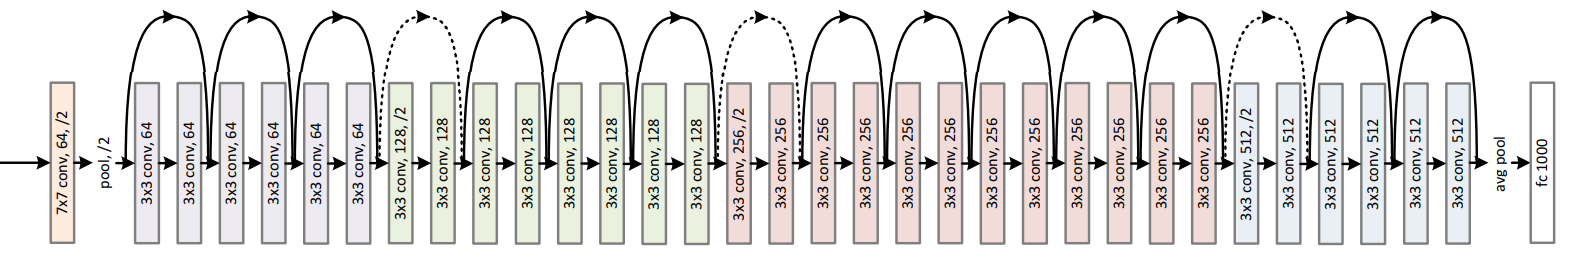
\includegraphics[width=1\textwidth]{resnet.png}
\end{figure}

\noindent We also used image augmentation for the model by using shift, rotation and flip for our images. These random transformations should make the dataset larger and make sure that you have the same images in different angles.\\

\subsection*{Milestones}

\ \\  \ \\
\noindent When we started our use case we made a plan what milestones we want to achieve. These are the objectives we had at the beginning:
\begin{enumerate} 
\item Preprocess the data
\item Create a model for transfer learning in Python
\item Create a Docker image for this model
\item Traine the model on GKE using TensorFlowJobs on CPUs
\item Save the trained model
\item Traine the model on GKE using TensorFlowJobs on GPUs, because it's much faster (about 15 times faster)
\item Distributed training on multiple pods
\item Serving the model with TensorFlowServing
\end{enumerate}


\subsection*{Technologies}
\ \\ \ \\
To create the model we used Tensorflow and Keras.\\
 For our containers we used Docker and Kubernetes for organisation. \\
To manage the pods we first wanted to use kubectl and ksonnet. Meanwile they changed in Kubeflow ksonnet to kustomize but in the end they also deleted kustomize, so we just used kubectl alone.\\
 To manage the Kubeflow Deployment we used the GCP console, gcould and gsutil.\\
The data we managed with PVC and saved it in a GCS bucket. \\
 For monitoring we used Tensorboard. \\
 In the end we managed the model with TensorFlow Serving in Jupyter Notebook.
\ \\
%%%%%%%%%%%%%%%%%%%%%%%%%%%%%%%%%%%%%%%%%%%%%%%%%%%%%
%\newpage
\section{Use Case Implementation}

\subsection*{Create the model}
\ \\  \ \\
We created the model for transfer learning in Python. \\
Therefore we used our ResNet-50 network.
\begin{lstlisting}
# Create the model for transfer learning using pretrained ResNet50
    print('>>>>>>>>>>>>>>>>>>>>>>>')
    print('Creating the model...')
    model = Sequential()
    
    model.add(ResNet50(    
      include_top=False,   
      weights=weights, 
      pooling='avg' 
    ))
    
    model.add(Dense(
      args.numclasses, 
      activation='softmax' 
    ))
    
    # Do not train the first layer in transfer learning
    if args.transferlearning:
        model.layers[0].trainable = False

    model.compile(
      optimizer=args.optimizer, 
      loss='categorical_crossentropy', 
      metrics=['accuracy'] 
    )
\end{lstlisting}
\subsection*{Create a Docker}
\ \\  
\begin{lstlisting}
#This container contains your model and any helper scripts specific to your model.
FROM python:3.7
FROM tensorflow/tensorflow:1.13.1-py3

COPY requirements_io.txt /opt/
RUN pip install -r /opt/requirements_io.txt

ADD model.py /opt/model.py
RUN chmod +x /opt/model.py

ENTRYPOINT ["python"]
CMD ["/opt/model.py"]
\end{lstlisting}

\subsection*{Training}
\ \\  \ \\
For the training we first used image augmentation and then trained the model:
\begin{lstlisting}    
# Image generators
    image_size = 224

    print('>>>>>>>>>>>>>>>>>>>>>>>')    
    print('Creating the image generators...')
    data_generator_no_aug = ImageDataGenerator(preprocessing_function=preprocess_input)

    data_generator_with_aug = ImageDataGenerator(preprocessing_function=preprocess_input,
                                       horizontal_flip=bool(args.hflip),
                                       vertical_flip=bool(args.vflip),
                                       rotation_range=args.rotation,
                                       width_shift_range = args.wshift,
                                       height_shift_range = args.hshift)

    train_generator_with_aug = data_generator_with_aug.flow_from_directory(
            working_train_dir,
            target_size=(image_size, image_size),
            batch_size=args.batchsize,
            class_mode='categorical')

    validation_generator = data_generator_no_aug.flow_from_directory(
            working_test_dir,
            target_size=(image_size, image_size),
            batch_size=args.batchsize,
            class_mode='categorical')

    # Train the model
    print('>>>>>>>>>>>>>>>>>>>>>>>')
    print('Starting the training...')
    history_aug = model.fit_generator(
            train_generator_with_aug,
            epochs=args.epochs,
            validation_data=validation_generator,
            shuffle=True,
            callbacks=[tensorboard])

\end{lstlisting}
\subsection*{Save the model}
\ \\  

\noindent With Keras we couldn't save the model directly to the bucket. So we saved it locally first and then send it to the bucket (copy2bucket). 
\begin{lstlisting}
    print('>>>>>>>>>>>>>>>>>>>>>>>')
    print('Saiving the model localy...')
    time_stamp = str(int(time.time()))
    model_name = 'top' + str(args.numclasses) + '-' + time_stamp + '.h5'
    model.save(model_name)
    

    print('>>>>>>>>>>>>>>>>>>>>>>>')
    print('Trying to copy the model to a bucket...')
    try:
        copy2bucket(model_name, args.exportdir)
    except Exception as e: 
        print(e)
    
    print('>>>>>>>>>>>>>>>>>>>>>>>')
    print('Trying to copy the logs to a bucket...')
    try:
        import pickle
        history_file = 'history-top' + str(args.numclasses) + '-' + time_stamp + '.pkl'
        with open(history_file, 'wb') as f:
            pickle.dump(history_aug.history, f)
        copy2bucket(history_file, args.exportdir)
        logs = os.listdir('/logs')
        for l in logs:
            copy2bucket('/logs'+l, args.exportdir)
    except Exception as e: 
        print(e)
\end{lstlisting}

\noindent The function that is used to copy  the saved model to the bucket:
\begin{lstlisting}
def copy2bucket(file, bucket):
    with file_io.FileIO(file, mode='rb') as i_f:
        with file_io.FileIO(os.path.join(bucket, file), mode='wb+') as o_f:
            o_f.write(i_f.read())
            print('Copied', file, 'to', bucket)
\end{lstlisting}

\subsection*{Results}
\ \\ 

\noindent After the training you can check the predicitions. We ran it on Jupyter Notebook. \\
Therefore we import the trained and saved model. Then we import the csv-file and select the top 10 painters.\\
\begin{figure}[H]
	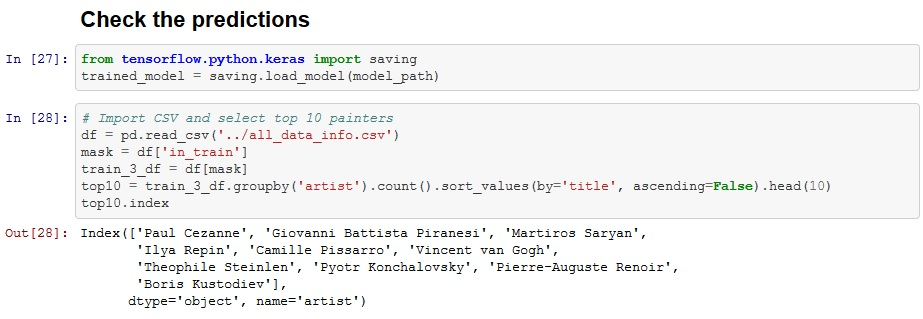
\includegraphics[width=1\textwidth]{Check1.jpg}
\end{figure}

\noindent  Then we select a random image of the input data and resize it to 224-by-224 pixels. \\
\begin{figure}[H]
	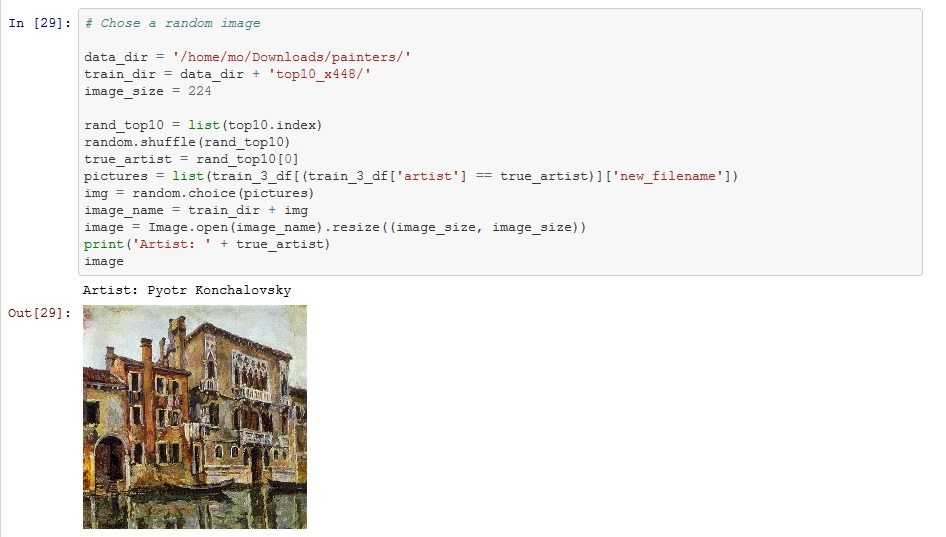
\includegraphics[width=1\textwidth]{Check2.jpg}
\end{figure}

\noindent In the end we get a display for the predicition of the model where the probability for each of the ten painters is shown in percent.\\
\begin{figure}[H]
	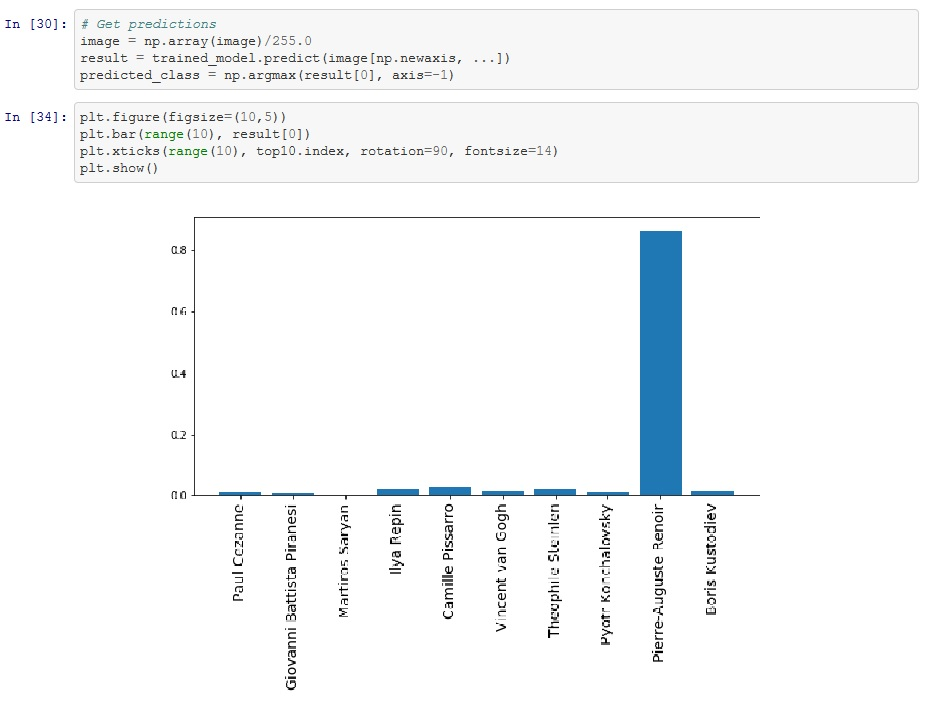
\includegraphics[width=1\textwidth]{Check3.jpg}
\end{figure}

\noindent Our model doesnt't give a good prediction for the 10 painters and it always shows the same prediction independently of the input image. That's because we just used a small amount of data for training so the model cannot give a proper prediction. 
 
\ \\ 
\subsection*{Problems}
\ \\  \ \\
\noindent One of our Problems was that we used Keras, but Keras cannot save models/logs directly to the bucket. We had to save it locally and then send it to the bucket. \\
Also there is no obvious support for distributed learning on one computer we could use. \\

\noindent Another problem was that we first tried to use Kustomize and then Ksonnet but they didn't work anymore.

%%%%%%%%%%%%%%%%%%%%%%%%%%%%%%%%%%%%%%%%%%%%%%%%%%%%%
\ \\
\section{Conclusion}

\noindent Keras simplifies the work with CNN models but it has several restrictions: \\
On the one hand Keras cannot work directly with GCS buckets. On the other hand Keras does not directly support distributed learning. \\

\noindent Tensorflow itself requires additional learning time if you want to use it.\\

\noindent In conclusion we can say that Kubeflow is still very raw. There are rapid changes and a low backward compatibility. Also you have to learn all underlying technologies like Kubernetes, Docker, Tensorflow.\\
Finally it's important to say that Kubeflow is a tool that is not for data science. It is for model training. \\

\noindent We only recommend it for machine learning and only for people that have experience or knowledge of the used tools in Kubeflow. Also we would recommend to use it more in the futur when Kubeflow is more sophisticated.
\ \\
% Literaturverzeichnis
%\cleardoublepage
%\phantomsection
\addcontentsline{toc}{chapter}{Literaturverzeichnis}
\bibliography{literatur}

\begin{thebibliography}{7}

\bibitem{1}
https://www.kubeflow.org/docs/

\bibitem{2}
https://github.com/kubeflow/examples

\bibitem{3} 
https://www.kaggle.com/c/painter-by-numbers/

\bibitem{4} 
Kaiming He, Xiangyu Zhang, Shaoqing Ren, Jian Sun. \textit{Deep Residual Learning for Image Recognition}, arXiv:1512.03385

\bibitem{5} 
https://keras.io/

\bibitem{6} 
https://www.tensorflow.org/guide

\bibitem{7} 
https://kubernetes.io/docs/

 
\end{thebibliography}
\end{document}
